\documentclass[11pt]{article}
\usepackage[utf8]{inputenc}	% Para caracteres en español
\usepackage{amsmath,amsthm,amsfonts,amssymb,amscd}
\usepackage{multirow,booktabs}
\usepackage[table]{xcolor}
\usepackage{fullpage}
\usepackage{lastpage}
\usepackage{enumitem}
\usepackage{fancyhdr}
\usepackage{mathrsfs}
\usepackage{wrapfig}
\usepackage{setspace}
\usepackage{calc}
\usepackage{multicol}
\usepackage{caption}
\usepackage{amssymb}
\usepackage{cancel}
\usepackage[retainorgcmds]{IEEEtrantools}
\usepackage[margin=3cm]{geometry}
\usepackage{amsmath}
\newlength{\tabcont}
\setlength{\parindent}{0.0in}
\setlength{\parskip}{0.05in}
\usepackage{empheq}
\usepackage{framed}
\usepackage[most]{tcolorbox}
\usepackage{xcolor}

\usepackage{color}
\definecolor{darkred}{rgb}{.8,0,0}
\definecolor{gray}{rgb}{.4,0.4,0.4}
\definecolor{blue}{rgb}{0,0,1}
\def\addMA#1{{\noindent\color{blue}{#1}}}


\colorlet{shadecolor}{orange!15}
\usepackage[colorlinks=true, allcolors=blue]{hyperref}
\parindent 0in
\parskip 12pt
\geometry{margin=1in, headsep=0.25in}
\theoremstyle{definition}
\newtheorem{defn}{Definition}
\newtheorem{reg}{Rule}
\newtheorem{exer}{Exercise}
\newtheorem{note}{Note}

\newcommand{\DD}{\textbf{D}}
\newcommand{\PP}{\textbf{P}}
\newcommand{\RR}{\textbf{R}}
\newcommand{\QQ}{\textbf{Q}}
\newcommand{\kk}{\langle k \rangle}


\begin{document}
%\setcounter{section}{8}
%\title{Chapter 9 Review Notes}

%\thispagestyle{empty}

%\begin{center}
%{\LARGE \bf Ptychography}\\
%%{\large Physics 300}\\
%%Fall 2016
%\end{center}
% ----------------------------------------------------------------
\title{\LARGE {\textbf{Statistical Modeling of X-ray Scattering Experiment in Low Photon Count Regime}}}
\maketitle
%\date{\today}
%\dedicatory{}%
% ----------------------------------------------------------------
\newpage
\section{X-rays Speckle Visibility Spectroscopy (XSVS)}
\subsection{What is speckle contrast/ visibility}
\label{subsec:speckle}
Speckle contrast, denoted as $\beta$, is a measure of the intensity variations in a speckle pattern, where bright spots result from constructive interference and dark spots from destructive interference of scattered X-rays. It depends on the coherence properties of the X-ray beam and the experimental configurations \cite{hruszkewycz_high_2012}. Speckle contrast is typically computed as the normalized variance of the intensity signal distribution at the detector given by $\beta = \sigma_I/\langle I \rangle$ \cite{hruszkewycz_high_2012}. Since speckle contrast reflects the extent to which the scattered waves interfere, it can also be expressed as the ratio of the difference between the maximum and minimum intensities to their sum, i.e., \(\beta = (I_{\text{max}} - I_{\text{min}})/( I_{\text{max}} + I_{\text{min}})\). Thus, the maximum achievable contrast is 1, occurring when the waves interfere perfectly constructively and destructively, creating sharp intensity variations. On the other hand, a contrast of 0 would imply no interference patterns, with uniformly distributed intensities. 

Several factors can reduce speckle contrast: if the coherence length of the incident beam is less than the illuminated volume of the sample, if the detector pixels are too large to resolve the speckle, or if the sample rearranges over the timescale during which the pattern is recorded \cite{hruszkewycz_high_2012}. 

A speckle pattern arises in the far-field from the interference between the wavefronts scattered from heterogeneities in the materials due to varying phase shifts being introduced into the scattering of coherent incident light. Speckle size \(s\) is dictated by the X-ray wavelength \(\lambda\), sample-to-detector distance \(D\) and illuminated area size \(d\) via the relationship \(s = \lambda D/d \). 

The evolution of the system can be captured by taking a time series of speckle patterns and quantifying the changes in speckles from frame to frame to study dynamics of materials from the rearrangements of speckle patterns. Speckle contrast captures the changes in the system that occurs within the data collection period of a single frame by utilizing the photon statistical properties of the detected photons in a X-ray scattering experiment. 

\subsection{Contrast in low-photon count limit}
\subsubsection{Negative Binomial analysis}
The fluctuations in the intensity distribution of a coherent beam is well approximated by gamma density function, and discrete photon counts on the detector follows a Poisson distribution \cite{goodman_speckle_2020}. Thus, the probability distribution of photons arriving in a single detector pixel k of a speckle pattern follows negative binomial (NB) distribution Eq. \ref{eqn:NB}, which is the convolution of gamma distribution with Poisson distribution \cite{goodman_speckle_2020}. The mean photon count (per pixel per pulse) is $\kk$, and the number of coherence modes in the speckle pattern is \( M \), where \(M \equiv \beta^{-1} \) \cite{hruszkewycz_high_2012}. It quantifies the degree of decoherence, which is influenced by the coherence length of the incident beam, detector pixel size, and sample dynamics. Speckle contrast is maximum at unity for single-mode distribution and decreases as M $\rightarrow \infty$ \cite{hruszkewycz_high_2012}. 
\begin{align}\label{eqn:NB}
P_{NB}(k) = \frac{\Gamma(k+M)}{\Gamma(M)\Gamma(k+1)} \left(\frac{\kk}{\kk+M}\right)^k \left(\frac{M}{\kk +M}\right)^M
\end{align}
Normalized variance of NB is the sum of gamma and Poisson distributions, given by Eq. \ref{eqn:NB_var}. The second term becomes significant at low count rates when $\langle k \rangle \ll$ 1, so tracking contrast using variance can be inaccurate. 
\begin{align}\label{eqn:NB_var}
M^{-1} = \frac{\sigma^2(k)}{\kk^2} - \frac{1}{\kk}
\end{align}
Instead, we can directly extract speckle contrast from the observed P(k) through the probability to detect 0, 1 or 2 photon events via Taylor series expansion for P(1) and P(2) \cite{hruszkewycz_high_2012}. Similarly, fitting the observed photon probabilities to Eq. \ref{eqn:NB} can determine \( M \) and thus, speckle contrast.
\subsubsection{Extension of NB analysis}

\section{XPCS}
\label{sec:XPCS}
\subsection{X-ray Photon Correlation Spectroscopy (XPCS)}
\label{subsec:xpcs}
XPCS is a statistical technique that utilizes the rearrangement of speckle to study materials dynamics as noted in Subsection \ref{subsec:speckle}. It quantifies these dynamics by correlating frame-to-frame speckle intensity variations over different time intervals (Eq. \ref{eqn:TTCF}) since distinctive speckle pattern arises when coherent X-rays scatters off a particular atomic arrangement within a sample \cite{jo_single_2023}. 

One analysis approach involves the two-time correlation function (TTCF). TTCF is an anti-symmetric 2D matrix by construction \cite{cao_effect_2020} and represents the cross-correlation of the intensity fluctuations separated by a certain time delay between all possible pairs of pulses (frames) (Fig. \ref{fig:xpcs_example}b). Rearrangement of speckle is reflected in the intensity fluctuations of the pixels at each frame. Thus, TTCF gives insight into how the system has evolved over the duration of the probe by keeping track of the speckle changes in each pixel over different frames. By performing the anti-diagonal sum of TTCF, which is the time-averaging over the similar time delays, correlation coefficients spanning various time delays is computed (Fig. \ref{fig:xpcs_example}c). This 1D correlation function, called \(g_2\) Eq. \ref{eqn:g2}, tells us the timescale of the system's decorrelation under a certain experimental condition. 
\begin{subequations}\label{eqn:TTCF_g2}
\begin{align}
\label{eqn:TTCF}
TTCF(Q, t_1, t_2) &= \frac{\left<I_{t_1} I_{t_2}\right>}{\left<I_{t_1}\right> \left<I_{t_2}\right>} \\
\label{eqn:g2}
g_2(Q, t_1, t_2) &= \frac{\overline{\left<{I}_{t_1} {I}_{t_2}\right>}}{\overline{\left<{I}_{t_1}\right>} \overline{\left<{I}_{t_2}\right>}} \\
&= 1 + \beta |f(Q, \Delta t)|^2
\end{align}
\end{subequations}
The $\left<.\right>$ denotes ensemble averaging of the pixels' intensities at an equivalent momentum transfer wave vector Q ($|\QQ| = \frac{4 \pi}{\lambda} \sin(\frac{\theta}{2}))$ for a chosen region of interest from speckle patterns, and the bar denotes the time averaging. The X-ray wavelength is $\lambda$, and the scattering angle is $\theta$. $\beta$ is the speckle contrast and $f(Q, \Delta t)$ is the intermediate scattering function, which contains information about the dynamics of the sample \cite{jo_single_2023}. For a simple mono-disperse colloidal systems that follow Brownian motion, this can be captured using an exponential decay function via the Stokes-Einstein relation \cite{jo_single_2023}.

In XPCS method, the repetition rate of the detector dictates the time resolution of the dynamical processes that can be captured \cite{jo_single_2023} while the duration of the X-ray pulse determines the timescale of the frozen snap shot that can be taken at each instance.
\begin{figure}[ht!]
    \centering
    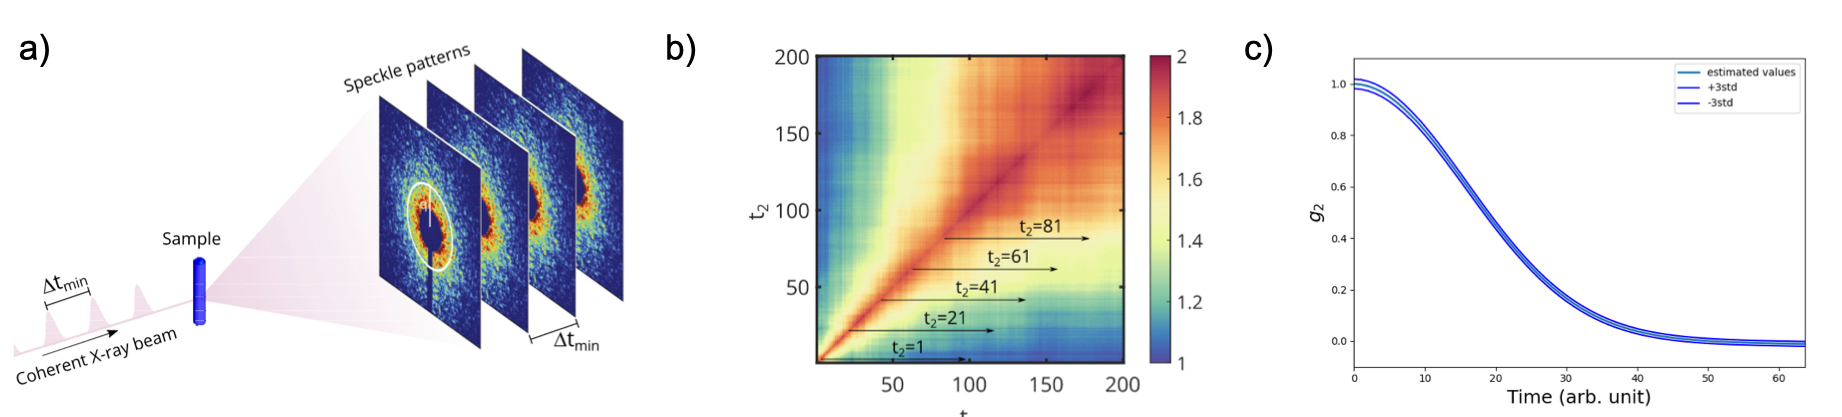
\includegraphics[width=165mm]{figures/xpcs_fig.001.jpeg}
    \captionsetup{font={small}, justification=centering}
    \caption{a) XPCS scheme in small-angle X-ray scattering geometry. b) Example 2D TTCF cross-correlation heat map between pairs of frames denoted $t_1$ (x-axis) and $t_2$ (y-axis). The black lines denoted with \(t_2 = 1, 21, 41\) and so on indicate one of the time pairs held constant as you go across horizontally on the TTCF heat map. (Figure a) \& b) from \cite{lehmkuhler_femtoseconds_2021}). c) Example \(g_2\) correlation function plot}
    \label{fig:xpcs_example}
\end{figure}
\subsubsection{Weighted TTCF}
One way to handle extreme fluctuations in recorded speckle intensities is by applying the similar weighting matrix via the equation \eqref{eqn:weightM} \cite{cao_effect_2020}. By applying this weighting matrix in computation of the TTCF, extremely weak shots will not contribute in calculating the correlation coefficient since $ w_{t_1}$ approaches 0 as $\left<I_{t_1}\right>$ approaches 0. Doing so will also help eliminate false correlations resulting from correlations between two extremely disproportionate pulses resulting from intensity fluctuations from X-ray sources. Thus, this weighted TTCF function discard pairs of pulses that are extremely weak or extremely strong and weak, consequently reducing the number of contributing pulses, in computation of the correlation coefficients.
\begin{align}\label{eqn:weightM}
w_{t_1, t_2} = \frac{n_{pix} \left<I_{t_1}\right> \left<I_{t_2}\right>}{\left<I_{t_1}\right> + \left<I_{t_2}\right> + 1}
\end{align}

\section{Variance of a Gamma/Gamma/Poisson random variable}
This section describes the underlying statistical model used to simulate an X-ray scattering experiment at a X-ray free electron laser (XFEL) source. 

A random variable (RV) is a function that maps from a set of all possible outcomes from a sample space to real-valued outcomes. Vectors in \(\mathbb{R}^n\) can be seen as functions defined on the set \(\{1, 2, \ldots, n\}\) mapping to real values. Specifically, a vector \(\mathbf{v} = [1, 2, 3]\) defines a function \(X\) such that \(X(i) = v_i\) for \(i \in \{1, 2, 3\}\). Here, \(\mathbf{v} = [v_1, v_2, v_3]\) and \(X: \{1, 2, 3\} \rightarrow \mathbb{R}\), where each index \(i\) maps to the corresponding vector component \(v_i\).

In this section, we derive the variance of a three-stage (compound) random variable (RV) driven as follow:  
%
\begin{itemize}

\item The first stage of the compound process is to draw two independent RV $X$ and $Y$ such that  
%
\begin{equation}
X \sim \mathcal{G}(1, L) 
\qquad \text{and} \qquad 
Y \sim \mathcal{G}(\mu, k)
\label{PDF_X}
\end{equation}
% 
with the following form of the Gamma probability distribution density (PDF) 
%
\begin{equation}
f_Y(y \,;\; \mu, k) = \frac{1}{\Gamma(k)}\frac{k}{\mu}\left(\frac{ky}{\mu} \right)^{k-1} e^{-\frac{k}{\mu}y}.
\label{PDF_Gamma}
\end{equation}
%
The statistical distribution of incoming X-ray intensity variations can be described by the Gamma distribution as shown in Eq.~\eqref{PDF_Gamma}. 
%
\addMA{%
With this parametrization, \(\mu\) represents the mean intensity, while the shape of the distribution \(k\) drives the variance of the RV since
%
\[
\text{VAR}[Y] := \langle (Y - \langle Y \rangle)^2\rangle = \frac{\mu^2}{k}.  
\]
%
}

%Note that the \(\mu\) parameter ultimately captures the mean photon density per pixel per frame of a diffraction pattern.
\begin{figure}[h!]
    \centering
    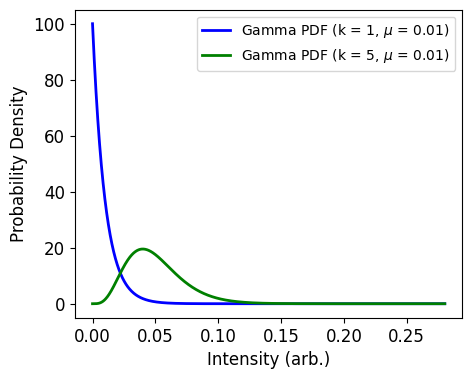
\includegraphics[width=70mm]{figures/gamma_pdf.png}
    \captionsetup{font={small}, justification=centering}
    \caption{Gamma PDF with the same mean and different shape parameter \(k = 1\) and \(k = 5\) denoted by purple and green respectively.}
    \label{fig:gamma_pdf}
\end{figure}

When \(k = 1\), the Gamma distribution simplifies to the negative Exponential distribution, Fig.\ref{fig:gamma_pdf}. This is analogous to the intensity fluctuations observed due a Self-Amplified Spontaneous Emission (SASE) process, where the SASE FEL intensity distribution exhibits a high frequency of extremely weak shots (causing the distribution to peak near zero) and infrequent shots where the intensity approaches the mean value. Likewise, for self-seeded FEL, \(k\) parameter would be greater than 1 with an intensity distribution that is more Gaussian\footnote{\addMA{It is actually a standard result that the Gamma PDF converges to the Gaussian PDF as $k$ grows, see for instance \cite[Sec. 3.3]{Goodman2007}}}r. This incoming X-ray intensity distribution is represented by the RV \(Y\). 

The Gamma RV \( X \) encapsulates two key aspects of an experiment: 
\begin{itemize}
    \item The mean of \( X \) represents the mean intensity due to sample dynamics, taking the role of a sample response function. While this mean need not be 1, it is inputted as 1 for simplicity.
    \item $L$ is a way to control the visibility of speckle of the recorded diffraction patterns. The physical phenomena that contributes towards reduction of visibility are: partial longitudinal and transverse, detector pixel size being too large to resolve speckle, and sample or beam instabilities. Thus, the inverse of L is the contrast of your system. 
\end{itemize}

Thus, the parameters \(\mu\), \( k \), and \( L \) approximately capture various distinct physical attributes of an X-ray beam and the experimental set-up that influence the dynamical parameters, such as the correlation coefficients, contrast and time constants of an X-ray scattering experiment. The RV \( X \) represents the combined effects of the sample dynamics, the coherence properties of the beam and imperfect experimental conditions, while RV \( Y \) captures the temporal fluctuations of the beam intensity.

\item The second stage is to define a second RV $Z$ that is the product of the two RV defined above, i.e., $Z:=X\times Y$. We have then
%
\begin{equation}
Z  \, \sim \, \mathcal{K}(\mu, k, L) 
\label{PDF_Z|Y}
\end{equation}
%
with the three-parameter $\mathcal{K}$-distribution 
defined as 
%
\begin{equation}
f_Z(z \,;\; \mu, k, L) = \frac{1}{\Gamma(k)\Gamma(L)}\frac{2kL}{\mu}\left(\frac{kLz}{\mu} \right)^{\frac{k+L}{2}-1} K_{L-k} \left[ \left( 2\frac{kLz}{\mu}\right)^{\frac{1}{2}}\right] .
\label{PDF_K}
\end{equation}
% 
where $K$ is the Bessel function of the second kind.
\begin{figure}[h!]
    \centering
    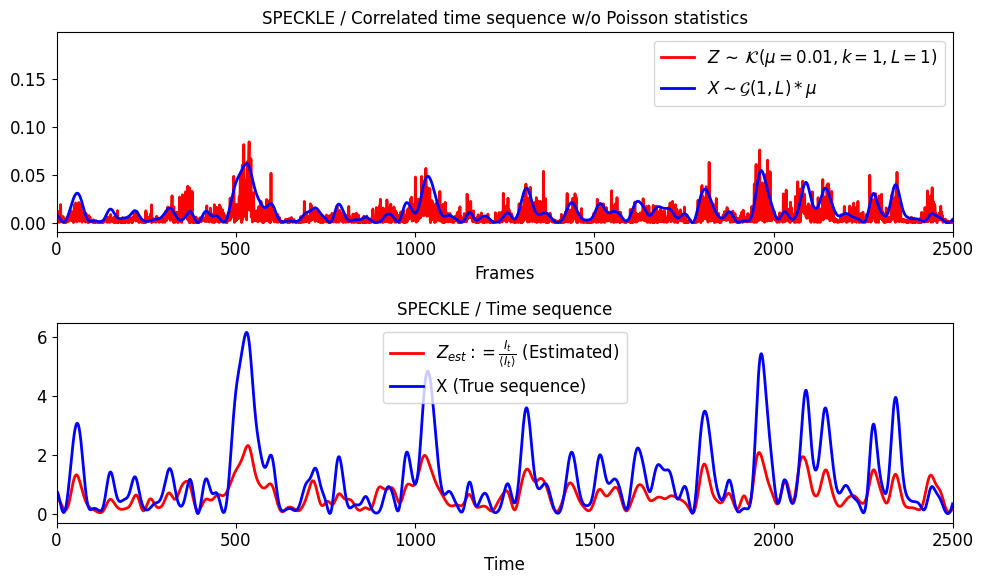
\includegraphics[width=120mm]{figures/speckl_noPoi_newlegend.png}
    \captionsetup{font={small}, justification=centering}
    \caption{Generated speckle time series of a single pixel with \(\mu = 10^{-2}\) mean photon count without Poisson counting statistics. Top: Intensity observed at the detector, RV \(Z\) (red) and input intensity RV \(X\) modulated by \(\mu\) (blue). Bottom: Ratio of recorded intensity pattern RV \(Z\) normalized by the mean of each frame (red) and the RV \(X\) (blue).}
    \label{fig:speckle_noPoi}
\end{figure}

The RV \(Z\), which is \(\mathcal{K}\)-distributed, is a product of the two functions that pertain to the sample response and the beam's temporal fluctuations and coherence properties. As such, its mean is the product of the sample response function's mean with beam intensity fluctuation distribution's mean and inherits the same shape parameters $k$ and $L$. It describes the statistical distribution of the intensity due to the interactions between the sample and the beam, \textbf{but without any Poisson photon counting statistics involved}, which means no discretization of photon counts have occurred yet, Fig.~\ref{fig:speckle_noPoi}. 
%
\item The third (and last) stage consist in drawing a Poisson RV $W$ with a mean parameter $\lambda$ driven by the value of the outcome $Z=z$, i.e.,
%
\begin{equation}
W \,|\, Z   \, \sim \, \mathcal{P}(\lambda = z).  
\label{PDF_Z|Y}
\end{equation}
%
\begin{figure}[h!]
    \centering
    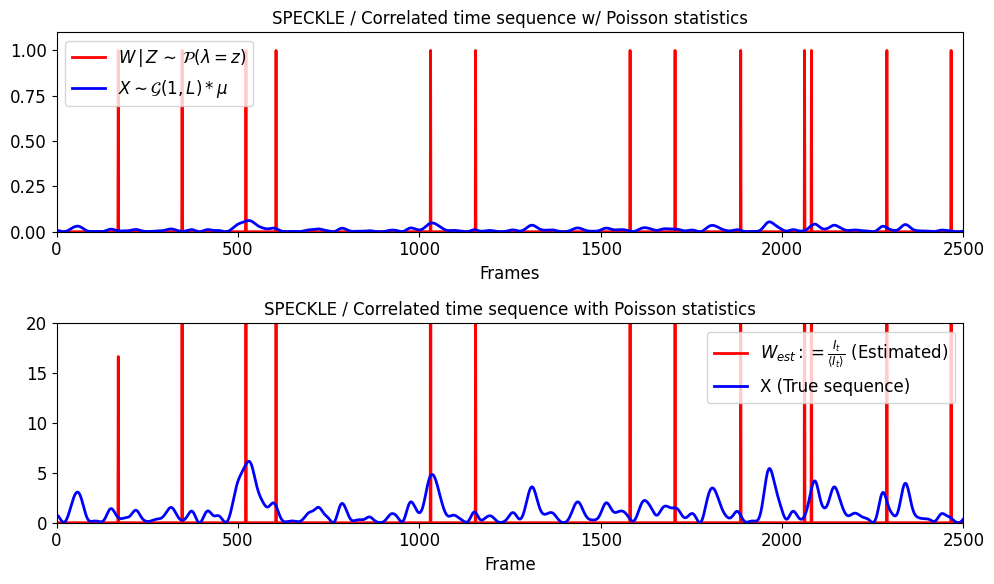
\includegraphics[width=120mm]{figures/speckle_poi_newlegend.png}
    \captionsetup{font={small}, justification=centering}
    \caption{Generated speckle time series of a single pixel with \(\mu = 10^{-2}\) mean photon count with Poisson counting statistics. Top: Intensity observed at the detector, \(W\) (red) and input intensity \(X\) modulated by \(\mu\) (blue). Bottom: Ratio of recorded intensity pattern \(W\) normalized by the mean of each frame (red) and the RV \(X\) (blue).}
    \label{fig:speckle_Poi}
\end{figure}
The last statistical distribution of this three-stage compound process incorporates Poisson statistics, Fig.~\ref{fig:speckle_Poi}. The statistical distribution of the number of photons detected in a given time interval on the detector can be modeled by a Poisson distribution. In the extremely photon-starved regime, Poisson counting statistics becomes prominent because it is rare to detect multiple photons within the time frame of a single data collection period. 
So \(W\) is a conditional probability distribution, describing the outcomes you would obtain with Poisson statistics involved once the outcomes from the product RV \(Z\) are considered. Consequently, \(W\) represents the intensity distribution of the diffraction patterns recorded, which is a direct observable in an experiment. 
\end{itemize}
%
Finally, we deduce the PDF of the observed XFEL-count $W$ by marginalizing the distribution of $(W,Z)$,  
%
\begin{equation}
f_W (\omega\, ;\, \mu,k,L) = \int f_{W|Z}(\omega\,|\,Z=z) \times f_Z(z;\mu,k,L)\, \text{d}z
\label{PDF_W}
\end{equation}
%
where the first and second PDFs under the integral are given by \eqref{PDF_Z|Y} and \eqref{PDF_K}, respectively.
An explicit form of this PDF can be found in \cite[Eq.~(4.3)]{Teich:89}. The explicit form of Eq. \eqref{PDF_W}, resulting from the convolution of \(\mathcal{K}\)-distributed RV \(Z\) with a Poisson distribution, which produces RV \(W\), is only necessary when we want to predict the distribution of intensity detected without specifying the value of the outcome \(z\). Since the knowledge of variance and expectation of \(W\) is sufficient to estimate the contrast of the system, we can use the two convolved distributions that make up \(W\) to compute the moments of \(W\) as follows.

We can compute the expectation and variance of $W$ \textit{via} the first two order moments of the Poisson  and $\mathcal{K}$ distributions. In particular, it is easy to derive from \eqref{PDF_W} and \eqref{PDF_Z|Y} that   
%
\begin{equation}
\begin{array}{rcl}
\langle W \rangle
&:=&\displaystyle \int \omega f_{W}(\omega) \, \text{d}\omega\\[1em]
&=&\displaystyle \int z f_{Z}(z;\mu,k,L) \, \text{d}z\\[1.2em] 
&\equiv& \langle Z \rangle. 
\end{array}
\label{mu_W_}
\end{equation}
The expectation of the conditional probability of Poisson RV \(W\) given \(Z = z\) depends on \(Z\). Therefore, the expectation of \(W\) is also the same as that of \(Z\). Intuitively, the convolution of a \(\mathcal{K}\)-distributed RV \(Z\) with a Poisson distribution preserves the mean of the \(\mathcal{K}\) distribution since Poisson statistics essentially discretize photon counts without changing the overall mean of the system.
%
The expectation of the $\mathcal{K}$-distributed
RV $Z$ \eqref{PDF_K} is $\mu$, which leads to 
%
\begin{equation}
\langle W \rangle  = \mu.
\label{mu_W}
\end{equation}
%
Similarly, it is not difficult to establish that 
%
\begin{equation}
\begin{array}{rcl}
\text{VAR}[W] &\equiv& \langle W^2 \rangle - \langle W \rangle^2\\[1em]
&=& \text{VAR}[\text{Poisson}(\mu)] + \text{VAR}[Z]\\[1em]
&=& \mu + \text{VAR}[Z]
\end{array}
\label{VAR_W_}
\end{equation}
Given \(W\) is the outcome of a Poisson process given the outcome of \(\mathcal{K}\) component, the variance of \(W\) should reflect both the intrinsic variance of \(\mathcal{K}\) and the Poisson process. For the Poisson distribution, the variance and mean are the same.
%
Because the variance of the RV $Z  \sim \mathcal{K}(\mu, k, L)$ is 
%
\begin{equation}
\begin{array}{rcl}
\text{VAR}[Z] &\equiv& \langle Z^2 \rangle - \langle Z \rangle^2\\[1em]
&=& \mu^2 \left( \frac{(k+1)(L+1)}{kL} - 1\right) 
\end{array}
\label{VAR_Z}
\end{equation}
%
we obtain
%
\begin{equation}
\text{VAR}[W] = \mu + \mu^2 \left( \frac{(k+1)(L+1)}{kL} - 1\right).
\label{VAR_W}
\end{equation}
We can retrieve \(L\) using Eq. \eqref{VAR_W} if we know the beam intensity distribution shape parameter \(k\), since estimate of \(\text{VAR}[W], ~\widehat{v}_W\), can be directly computed from the recorded diffraction patterns. Similarly, the product \(kL\) can be determined if \(k\) is unknown. The parameter \(k\) can be estimated by fitting a Gamma distribution for its shape parameter from the histogram constructed using the recorded incoming X-ray intensities, which is already something you record in an X-ray scattering experiment.  
%
For the usual (fully coherent) case $L=1$, this relation reads 
%
\begin{equation}
L=1 \quad \Rightarrow \text{VAR}[W] = \mu + \mu^2 \left( \frac{2}{k} + 1\right).
\label{VAR_W__}
\end{equation}
%
Finally, the general relation \eqref{VAR_W} can be used to derive a (moment-based) estimate for the parameter $L$. More specifically, an estimator for $L$ reads    
%
\begin{equation}
\widehat{L} \, := \, \frac{\mu^2(1 + k)}{k(\widehat{v}_W - \mu)- \mu^2}
\label{MomEst_L}
\end{equation}
%
where $\widehat{v}_W$ is the usual empirical variance computed from a series of outcomes of the RV $W$. 
 
In summary, this statistical model based on the three-stage compound process captures the various stochastic processes involved in an XRD experiment. It incorporates the fluctuations induced by the X-ray beam and the sample, as well as a way to control the visibility of speckle that affect the dynamical quantities of interest. In particular, the variance of these combined processes is crucial for extracting contrast as in Eq. \eqref{VAR_W}.

More specifically, Eq. \eqref{MomEst_L} estimates the contrast of the underlying system where the reciprocal of \(\widehat{L}\) represents the system's contrast, which is the intercept of the correlation coefficient function at \(\Delta t = 0\). This approach overcomes the need to detect two-photon events and to bin data based on incident beam intensity to account for the beam intensity fluctuations, because the analysis take into account of all pixels and how they evolve over time. Consequently, it allows for every shot to contribute towards the contrast estimate easily, enabling the extraction of contrast even with extremely low mean photon count rates, further lowering the detection limit. So far in theory :')

\section{Correlation Coefficients in XPCS}
%\subsection{\textbf{What is ptychography}}

Let \(I(t)\) be the intensity recorded in a given pixel at time $t$. We can compute the correlation of \(I(t)\) with $I(t+\tau)$ after some time delay \(\tau\) the following way %if \(I(t)\) is staionary:
\begin{align}\label{eqn:R1}
R^{(1)}_{t, t+\tau} := \frac{\left< I(t) I(t+\tau) \right>} {\left<I(t)\right>^2} .%\quad \text{where} \quad \overline{I}:= \left<I \right> 
\end{align}
%
Note that \(\langle \cdot \rangle\) denotes the expectation operator (i.e., the ensemble averaging). 
%
In practice, an estimation of this expectation is obtained by averaging the camera pixels over the user defined ROI, and
over various sets of pulse trains provided during the XFEL experiment.

%i.e., averaging across (ROI) pixels and bar denotes time averaging over equivalent \(\tau\). 

%\textit{Remove equiv bar and $<.>$, angle bracket: ROI averaging, bar: time averaging over equiv tau and update eqs. accordingly}

If $\langle I(t)\rangle$ is actually changing w.r.t time (e.g., in the XFEL SASE mode), we need to adapt the relation above 
%
\begin{align}\label{eqn:R2}
R^{(2)}_{t, t+\tau} := \frac{\left< I(t) I(t+\tau) \right> }{\left<I(t)\right> \left<I(t+\tau)\right>} =
\left\langle 
\frac{I(t)}{\langle I(t)\rangle}
\frac{I(t+\tau)}{\langle I(t+\tau)\rangle}
\right\rangle,
\end{align}
%
the second equality holding because of the linearity of the expactation operator.
%
The Eq.~\ref{eqn:R2} is the same as the TTCF equation in XPCS literature. 
%\textit{Eq. 2 is the same as TTCF}
\addMA{%
For notational simplicity, let $I(t) \equiv X$ and $I(t+\tau) \equiv Y$ so that Eq.~\ref{eqn:R2} takes a more compact form
%
\begin{align}
R^{(2)}_{X,Y}  = \frac{\langle XY\rangle}{\langle X\rangle\langle Y\rangle} = \left \langle \frac{ X}{\langle X\rangle} \frac{Y}{\langle Y\rangle} \right \rangle
\label{eqn:Rtt}
\end{align}
%
As we explain below, $R^{(1)}$ or $R^{(2)}$ are not the usual correlation coefficient as defined in applied statistics.  
}

\section{Correlation Coefficients in Statistics}
%
%For notational simplicity, let $I(t) \equiv X$ and $I(t+\tau) \equiv Y$. Then 
%
We introduce the correlation coefficient as it is defined in the statistical literature \cite[Sec. 27.8]{Kendall63_2a} as
%
\begin{align}
R_{X, Y} &:= \frac{\text{Cov}(X, Y)}{\sigma_X \sigma_Y} \label{eqn:Rxy1}
\end{align}
%
where $\text{Cov}(X,Y):= \left < (X - \left<X\right>) (Y- \left<Y\right>) \right>$ and $\sigma_X = \sqrt{\text{Var} (X)} 
%= \sqrt{\left < (X - \left<X\right>)^2 \right>}
$. 
%
Since $\text{Cov}(X,Y)$ can also be defined as $\text{Cov}(X,Y) = \left < X Y \right> - \left<X\right> \left<Y\right>$ the correlation coefficient above also reads 
%
\begin{align}\label{eqn:Rxy2}
R_{X,  Y} := \frac{\left < XY \right >}{\sigma_X \sigma_Y} - \frac{\left<X\right> \left<Y\right>}{\sigma_X \sigma_Y}.
\end{align}
%
%With the previous notation introduced for the XPCS experiment, we then have   
% 
%The standard correlation between two RV \(I(t)\) and \(I(t+\tau)\) are: 
%
%\begin{align}
%R_{I(t), I(t+\tau)}  = \frac{\text{Cov}(I(t), I(t+\tau))}{\sigma_{I(t)} \sigma_{I(t+\tau)}}
%= 
%\frac{\langle I(t) I(t+\tau) \rangle}{\sigma_{I(t)} \sigma_{I(t+\tau)}} - \frac{\langle I(t)\rangle \langle I(t+\tau)\rangle}{\sigma_{I(t)} \sigma_{I(t+\tau)}}.
%\label{eqn:Rtt}
%\end{align}
%
%Eq. \ref{eqn:Rxy1} is an alternative way to construct an element of 2D correlation matrix, TTCF. 
%\textit{Add another eq in Eq. 3 without replacing X and Y. Make the point this is another way to make an element of TTCF}\\
%\textit{Keep bar and $<.>$ notation the same as above}
%
How does subtracting the mean (ROI) pixels intensity of each frame, \(\left<X\right>\), from each corresponding recorded pixel intensity at time $t$, \(X\), before computing correlation coefficients compares to other XPCS methods or affect the resulting correlation coefficients? \addMA{[Should we suppress this paragraph? (it cannot be understood without knowing that the mean of a exponential RV is equal to its STD, which is stated in the next section).]}

%\textit{Let's contrast this each mean subtraction at each time with how other XPCS methods have done so. This is another way to get an element of TTCF. Eq. 3 and 4 same. put Eq 4 = $cos\theta$}
Important property of this correlation coefficient is that it satisfies similar properties as an inner product. If two random variables $X$ and $Y$ are of zero mean, then $\text{Cov}(X,Y)$  is the dot product of $X$ and $Y$, where the "length" of $X$ and $Y$ is $\sigma_X$ and $\sigma_Y$ respectively and thus, the correlation is the cosine of the angle between two vectors. That is:
\begin{align}
R_{X, Y} &= \frac{X \cdot Y}{\|X\| \|Y\|} = \frac{\text{Cov(X,Y)}}{\sigma_X \sigma_Y} = \cos(\theta)\label{eqn:covdot}
%\text{Cov(X,Y)} &= \sigma_X \sigma_Y \cos(\theta)
\end{align}
This means correlation Eq.~\ref{eqn:Rxy2} is a measure of similarity between random variables. From Cauchy-Schwartz inequality \addMA{[REF]}, which states that the absolute value of the dot product of two vectors is less than or equal to the product of the norm of the two vectors, we have
\begin{align*}
    |\text{Cov(X,Y)}| \leq \sigma_X \sigma_X
    \iff -1 \leq R_{X,Y} \equiv \frac{\text{Cov}(X, Y)}{\sigma_X \sigma_Y} \leq 1.
\end{align*}
%\textit{How does it go from left inequality to the right upper and lower bound. Max. corr value you can obtain is 1 in this construction. Which is different than traditional TTCF}
\addMA{%
Clearly, Eq.~\ref{eqn:Rxy1} is an alternative way to construct an element of 2D correlation matrix, TTCF.
%
For uncorrelated random variables $(X,Y)$, $\text{Cov}(X,Y) = 0$, hence,  $R_{XY}$ = 0 and the maximum correlation value you can obtain is 1 in this construction, different than as in time-averaging of TTCF to obtain \(g_2\). 
}
\section{Relationship between the two correlation coefficients}
So how is the correlation coefficient used in XPCS analysis,  $R^{(2)}_{XY}$ \eqref{eqn:R2},  related to the statistical correlation coefficient, $R_{XY} \eqref{eqn:Rxy2}$?

First, let us establish the following relations between the standard deviation $\sigma_X$ and its mean \(\left <X \right>\) for a given probability distribution function (PDF). PDF of pure speckle follows negative exponential, so its mean = standard deviation. Pure speckle, \(R_{XY}^\text{SPE}\), implies an element of the traditional 2D correlation TTCF matrix in XPCS analysis. 

For independent r.v. X and Y, the variance of their sum or difference is the sum of their variances. Thus, when you include Poisson photon counting statistics to pure speckle case, we can simply add the respective variances from each PDF and square root that quantity to obtain the standard deviation of the combined PDF.   

\begin{table}[h!]
\centering
\begin{tabular}{|c|c|c|c|}
\hline
PDF for $X$ & Speckle & Poisson & Speckle/ Poisson \\
\hline
Mean & $\left<X\right>$ & $\left<X\right>$ & $\left<X\right>$ \\
\hline
$\sigma_X$ & $\left<X\right>$ & $\sqrt{\left<X\right>}$ & $\sqrt{\left<X\right> + \left<X\right>^2} = \left<X\right> \sqrt{(1 + \frac{1}{\left<X\right>})}$  \\
\hline
\end{tabular}
%\caption{Table}
\label{tab:mytable}
\end{table}

The usual statistical correlation coefficient, $R_{XY}$ \eqref{eqn:Rxy2}, reads under each PDF assumption given in the table:
\begin{itemize}[label=$\diamond$]
    \item Speckle, negative exponential $\left(\sigma_X = \left<X\right>\right) \implies R_{XY} = \frac{\left< X Y \right>}{\left<X\right> \left<Y\right>} - 1 \equiv R_{XY}^\text{SPE}$
    \item Poisson $\left(\sigma_X = \sqrt{\left<X\right>}\right) \implies R_{XY} = \frac{\left< X Y \right>}{\sqrt{\left<X\right> \left<Y\right>}} - \sqrt{\left<X\right>\left<Y\right>} \equiv R_{XY}^{\text{SPE}}  \sqrt{\left<X\right> \left<Y\right>}$
    \item SPE+Poisson $\left(\sigma_X = \sqrt{\left<X\right>^2 + \left<X\right>} \right) \implies R_{XY} = R_{XY}^{\text{SPE}} \left(1+\frac{1}{\left<X\right>}\right)^{-1/2} \left(1+\frac{1}{\left<Y\right>}\right)^{-1/2}$
\end{itemize}
%\textit{Pure speckle = Traditional XPCS TTCF matrix element}
To summarize: 
\begin{align}
\alpha(\left<X\right>, \left<Y\right>) &= 1 & \text{if PDF = SPE} \\
\alpha(\left<X\right>, \left<Y\right>) &= \sqrt{\left<X\right>\left<Y\right>} & \text{if PDF = Poisson} \\
\alpha(\left<X\right>, \left<Y\right>) &= \left(1+\frac{1}{\left<X\right>}\right)^{-1/2} \left(1+\frac{1}{\left<Y\right>}\right)^{-1/2} & \text{if PDF = Speckle + Poisson}
\end{align}
Since $R_{XY}^{\text{SPE}} := \frac{\left\langle XY \right\rangle}{\left<X\right> \left<Y\right>} - 1$, when considering SPE+Poisson case:
%\section{\textbf{Putting it all together}}
\begin{align}\label{eqn:Rxy2_final}
R^{\text{SPE}}_{X Y} \equiv \frac{\left< XY \right>}{\left<X\right>\left<Y\right>} = 1  + \frac{R_{XY}}{\alpha (\left<X\right>, \left<Y\right>)}
\end{align}
Using XPCS notation: 
\begin{align}
\label{eqn:xpcs_corr}
\begin{split}
R^{(2)}_{t, t+\tau} &:= \frac{\left< I(t) I(t+\tau) \right> }{\left<I(t)\right> \left<I(t+\tau)\right>} \\
&= 1 + \frac{R_{I(t), I(t+\tau)}}{\alpha \left(\left<I(t)\right>,\left<I(t+\tau)\right>\right)}
\end{split}
\end{align}

\section{Numerical Simulation of an X-ray Scattering Experiment}

%\begin{GrayBox}
%\begin{verbatim}
%>> cp ../phase-separation-tutorial.tar.gz .
%>> tar -zxvf phase-separation-tutorial.tar.gz
%>> cd phase-separation-tutorial
%\end{verbatim}
%\end{GrayBox}
%\subsection{\textbf{Definitions}}
%
%\begin{list}{\color{black}$\heartsuit$}{\color{blue}}
%\item Statistical inference: parametric estimation
%\item Unbiased: systematic-error free estimation
%\item Minimal variance: efficient estimator
%\item Maximum likelihood: method of estimating the parameters of an assumed probability distribution by maximizing a likelihood function so that, under the assumed statistical model, the observed data is most probable.
%\end{list}
%
%\section{\textbf{Negative Binomial Distribution}}
%
%\begin{align}\label{eqn:nb}
%f(y; \lambda, M) &= \frac{\Gamma(y+ M)}{\Gamma(M) \Gamma(y+1)} \left(\frac{\lambda}{\lambda + M}\right)^{y} \left(\frac{M}{\lambda + M}\right)^M\\
%&= \frac{\Gamma{(y+M)}}{\Gamma{(M)}\Gamma{(y+1)}} \left(1+\frac{M}{\lambda}\right)^{-y} \left(1+\frac{\lambda}{M}\right)^{-M} \nonumber
%\end{align}





 


\bibliographystyle{plain}
\bibliography{refs_photon_stats}

\end{document}
% ----------------------------------------------------------------

A random variable (r.v.) is a function that maps from a set of all possible outcomes from a sample space to real-valued outcomes. Vectors in \(\mathbb{R}^n\) can be seen as random variables on the probability space \(\{1, 2, \ldots, n\}\). That is, r.v. are functions defined on the set \(\{1, 2, \ldots, n\}\) mapping to real values. Specifically, \(\mathbf{v} = [1, 2, 3]\) defines a function \(X\) such that \(X(i) = v_i\) for \(i \in \{1, 2, 3\}\). Here, \(\mathbf{v} = [v_1, v_2, v_3]\) and \(X: \{1, 2, 3\} \rightarrow \mathbb{R}\), where each index \(i\) maps to the corresponding vector component \(v_i\).

a vector in \(mathbb{R}^n\) as a function that takes the sequential number of an element of the probability space as input, and gives a real number as output. This matches the definition of a real random variable over that probability space, which is a function that maps each element of the probability space to a real number